

\section{基于eBPF的DPU静态虚拟化}

云计算技术对异构需求越来越高,传统架构存在着处理能力与数据量增长不匹配、资源利用不足、安全风险等问题。DPU功能serverless化变得非常常见。例如英伟达推出的DOCA平台框架(DPF)是一个DPU程序编排框架,帮助创建BlueField加速的云软件平台,使得DPU可以在K8s环境中被直接使用。同时已有研究人员开始研究异构计算系统(CPU-GPU-DPU)上的serverless系统(Serverless Computing on Heterogeneous Computers ASPLOS’22)。

DPU 容器(DPU container)通常是指基于 DPU(数据处理单元)技术,使用容器化技术来部署和管理的计算环境。简单来说,它结合了 DPU 的硬件加速能力和容器的灵活性,通常用于高性能计算、网络加速、存储加速等场景。
Nvidia DPU具有硬件级隔离:NVIDIA BlueField DPU通过硬件加速引擎和专用处理资源,为每个租户提供独立的计算、存储和网络资源,确保租户之间的资源隔离。在云原生计算平台中,DPU通过卸载和加速基础设施功能,支持多租户环境下的高性能计算。DOCA编程框架(DPF)可以实现多租户的DPU服务的调配和编排,通过容器化的方式将 Kubernetes 控制平面功能扩展到 DPU,使管理员能够直接在 BlueField DPU 上部署和卸载 NVIDIA DOCA 服务和基于 DOCA 的第三方服务。DPF 配备了专门用于无缝集成的 SDK,提供了一个一致的模块化工具包,例如OVS,RDMA开发工具包。

\captionsetup[figure]{justification=justified}
\begin{figure}
	\centering
		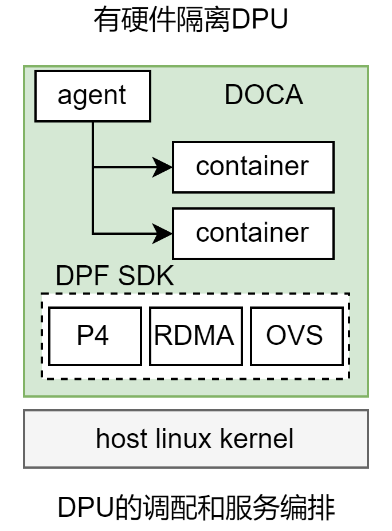
\includegraphics[width=0.3\textwidth]{figures/figure2}
 \label{fig:diagram}
 \caption{DPU 应用程序的调配和服务编排}
 
%  \captionwithsource{热塑性形状记忆聚氨酯的形状记忆机理示意图}{数据来源:交代图形的出处或者来源,示明“作者、来源名称、时间”,用小五宋体,置图左下方。交代图形的出处或者来源,示明“作者、来源名称、时间”,用小五宋体,置图左下方。}
\end{figure}

目前国内的 DPU(数据处理单元)在硬件级隔离方面的能力相对有限,要实现完全的硬件级隔离(特别是在安全性、可靠性、性能等方面的完全隔离)仍需要进一步的技术发展和硬件支持,尤其是是在K8s等云应用场景下。

1.虚拟化和资源隔离:许多 DPU 提供了硬件加速的虚拟化支持,尤其是在网络、存储和计算资源的隔离方面。例如,DPUs 如浪潮的“云脉”DPU或者华为的“昇腾”DPU,已经具备一定的隔离能力,能够在同一物理硬件上支持多个虚拟机或容器的运行,并为其提供网络加速、存储加速等服务。但这种隔离更多是针对资源访问的虚拟化层面的,而非完全的硬件隔离。

2.安全性与可信计算:要实现完全的硬件级隔离,还需要依赖于更强的安全特性,比如硬件级的加密、完整性保护、物理隔离等机制。目前一些 DPU 已经支持基于硬件的安全功能(如加密引擎),但对于极高要求的安全场景(如政府、金融等领域),硬件级的完全隔离通常需要结合特殊的硬件设计和安全协议,甚至依赖于可信执行环境(TEE)技术。

3.DPU与CPU的协同工作:目前的 DPU 在硬件级的完全隔离方面,可能仍然受到 CPU 和内存共享、I/O 访问控制等因素的制约。尤其是在一些复杂的并发计算和高性能计算场景下,虽然 DPU 可以通过硬件支持高效的网络处理和计算加速,但要完全独立于 CPU 的安全和资源调度依然是一个技术难点。

目前国内的这种不具备完全硬件隔离能力的DPU无法支持租户之间的资源隔离要求,阻碍了DPU容器化的应用。
ebpf 借助ebpf verfier实现了一个安全的沙箱,可以防止ebpf代码以多种方式来损害内核(DOS攻击、信息窃取攻击等)。Verifier可以在一定程度上对容器内的代码实现安全性隔离(todo:需要找一些case分析)。同时,eBPF verifier运行在程序加载阶段,不会给函数容器启动添加额外影响。 通过ebpf verifier实现ebpf sandbox可以在软件层面对用户代码实现安全保障作用。加入ebpf sandbox后的DPU容器化模型如下图所示:

\captionsetup[figure]{justification=justified}
\begin{figure}
	\centering
		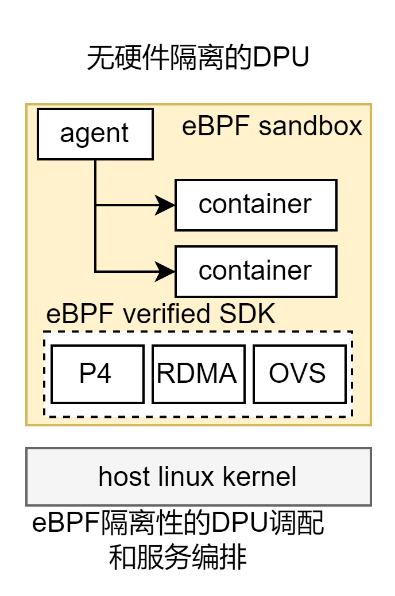
\includegraphics[width=0.3\textwidth]{figures/figure3}
 \label{fig:diagram2}
 \caption{eBPF隔离的DPU调配和服务编排}
 
\end{figure}

1. 硬件虚拟化与资源分区
SR-IOV(单根I/O虚拟化)
DPU的物理网卡通过SR-IOV虚拟化为多个虚拟功能(VF),每个租户的虚拟机(VM)或容器独占一个VF,实现网络流量的直接硬件隔离,减少延迟并提升吞吐量。

硬件资源分片
DPU的计算核心(如Arm CPU、加速引擎)和内存资源通过硬件分区分片,为不同租户分配独立的计算单元和内存空间,防止资源争用。 

\subsection{系统设计与实现}

\subsubsection{总体架构设计}

本方案采用分层架构(如图X-1所示),核心模块包括 静态验证器、白名单管理器、资源隔离引擎 和 回退控制器。系统工作流程如下:

1.用户提交函数代码后,触发静态验证器进行内存安全与行为合规性检查。
2.验证通过的函数以普通进程形式运行,由资源隔离引擎限制其权限与资源使用。
3.验证失败的函数触发回退控制器,启动容器实例执行,同时记录失败原因供后续优化。
4.白名单管理器动态维护安全函数列表,支持按需扩展与权限分级。


\subsection{ 核心模块设计}

\subsubsection{静态验证器}

目标:确保函数代码无内存越界、非法控制流与未授权系统调用。
实现方案:

中间表示(IR)生成:基于LLVM将用户代码转换为IR,消除语言特性差异(如指针运算)。

安全规则检查:

内存安全:验证所有内存访问边界(如数组索引、缓冲区大小)。

控制流完整性:禁止跳转至动态计算地址(如函数指针需静态绑定)。

系统调用过滤:通过符号执行检测代码是否仅调用白名单函数。

形式化验证增强:集成Z3求解器,对循环与分支路径进行数学证明。
约束:强制使用预定义内存池(禁止malloc/free),支持Rust等内存安全语言优先通过验证。

\subsubsection{白名单管理器}

目标:提供最小化、场景化的安全函数集合。
实现方案:

分层白名单:

基础类:数学运算、字符串处理(如memcpy需带长度参数)。

I/O类:受限文件读写(仅限临时目录)、网络请求(过滤目标IP)。

平台服务类:访问数据库、消息队列的SDK封装。

动态审核机制:

社区投票新增高危函数(如execve),默认隔离至WebAssembly沙盒执行。

自动监控函数使用频率与安全事件,动态降级或移除风险项。

\subsubsection{资源隔离引擎}
目标:在普通进程模式下实现近似容器的隔离性。
实现方案:

轻量级隔离:

命名空间(Namespace):隔离进程视图(PID、网络、文件系统)。

cgroups:限制CPU、内存、磁盘IO配额。

安全加固:

seccomp策略:仅允许白名单内的系统调用(如禁止ptrace)。

SELinux上下文:为进程分配最小权限标签(如禁止写入/proc)。

硬件辅助:可选启用Intel SGX加密敏感数据内存区域。

\subsection{关键流程设计}

\subsubsection{函数提交与验证流程}

用户上传函数代码及依赖声明。

静态验证器执行多阶段检查:

阶段1(语法分析):检测禁用语言特性(如内联汇编)。

阶段2(符号执行):遍历所有代码路径,标记潜在越界访问。

阶段3(形式化证明):对不确定路径调用Z3验证安全性。

生成验证报告,通过则编译为可执行文件,否则触发回退流程。

\subsubsection{进程/容器混合调度流程}
资源调度器根据验证结果分配执行环境:

进程模式:直接调用fork()启动,附加cgroup、seccomp策略。

容器模式:从预热池选取镜像,通过runc启动实例。

资源监控器实时收集CPU、内存指标,超限时强制终止进程或扩容容器。
